\chapter{\heiti 软件使用}
\section{\heiti 打开控制软件}
进入我司为用户提供的“Integration”的文件夹,双击运行“ASG.py”文件,即可打开包含图形用户界面的仪器控制软件。软件主界面(Pulse界面)如图4-1所示。
\begin{figure}[ht]
\centering
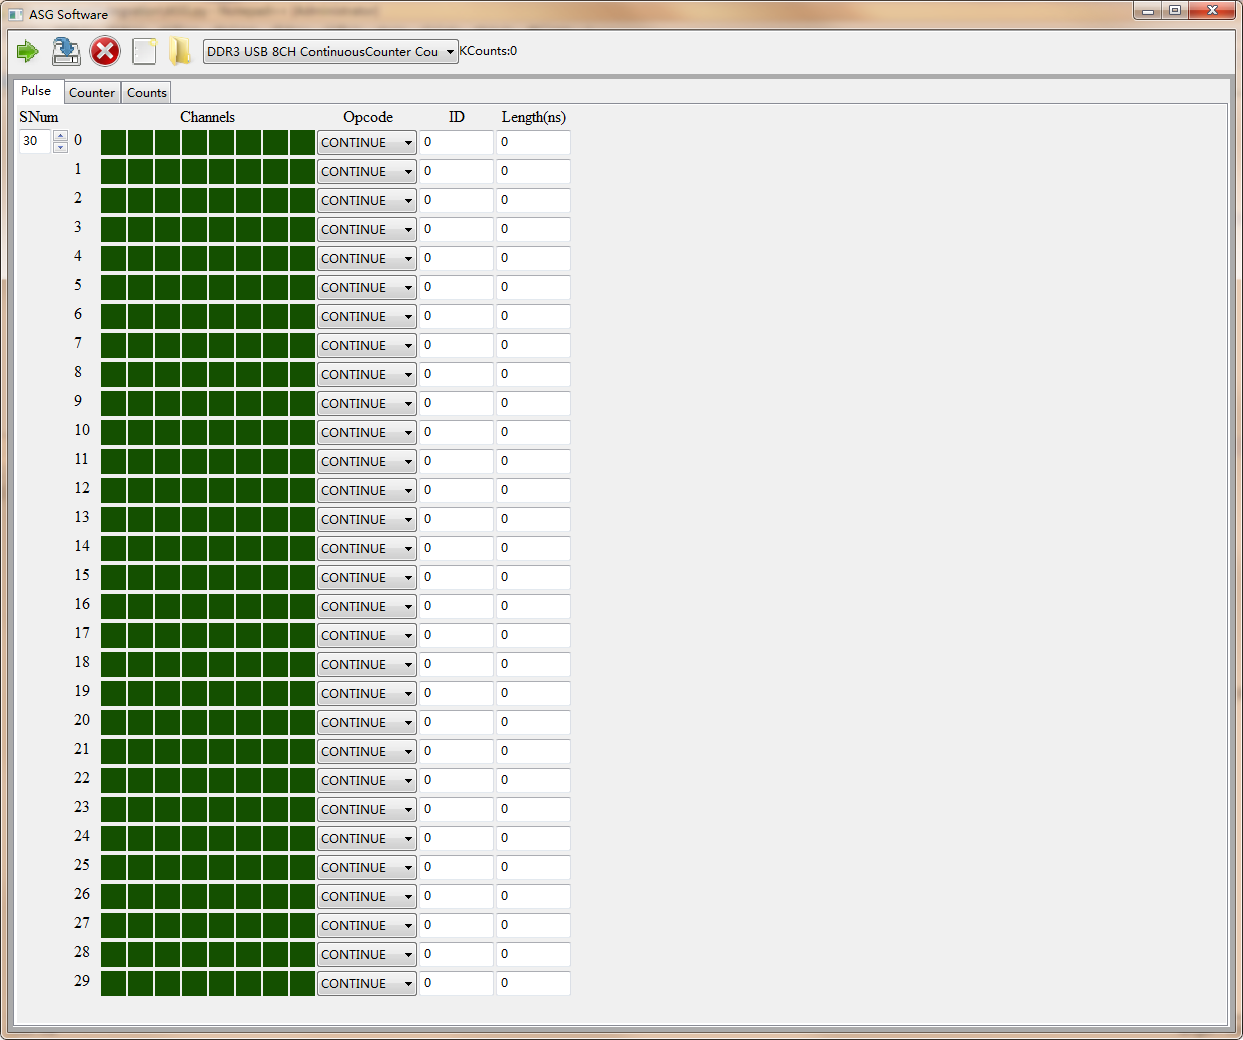
\includegraphics[width=12cm,height=10cm]{fig4_1}
\caption{软件主界面}
\end{figure}

在软件主界面中,每行8个绿色方框,从左往右依次代表OUT 1至OUT 8的8个方波输出通道在一段时间内的输出状态(时间长短由右侧的“Length”文本框内输出的数据决定,单位为纳秒)。当绿色被点亮时,该通道输出高电平;若绿色未被点亮,则代表该通道输出为低电平。

\section{\heiti 定义任意方波序列}
用户可以根据每行的绿色方框不同状态及“Length”的长度来定义任意的方波序列。例如用户想要在1、2、3、4通道生成一个高电平宽度为60 ns的方波序列,而5、6、7、8通道在这60 ns内为低电平。则可以如图4-2定义方波序列:
\begin{figure}[ht]
\centering
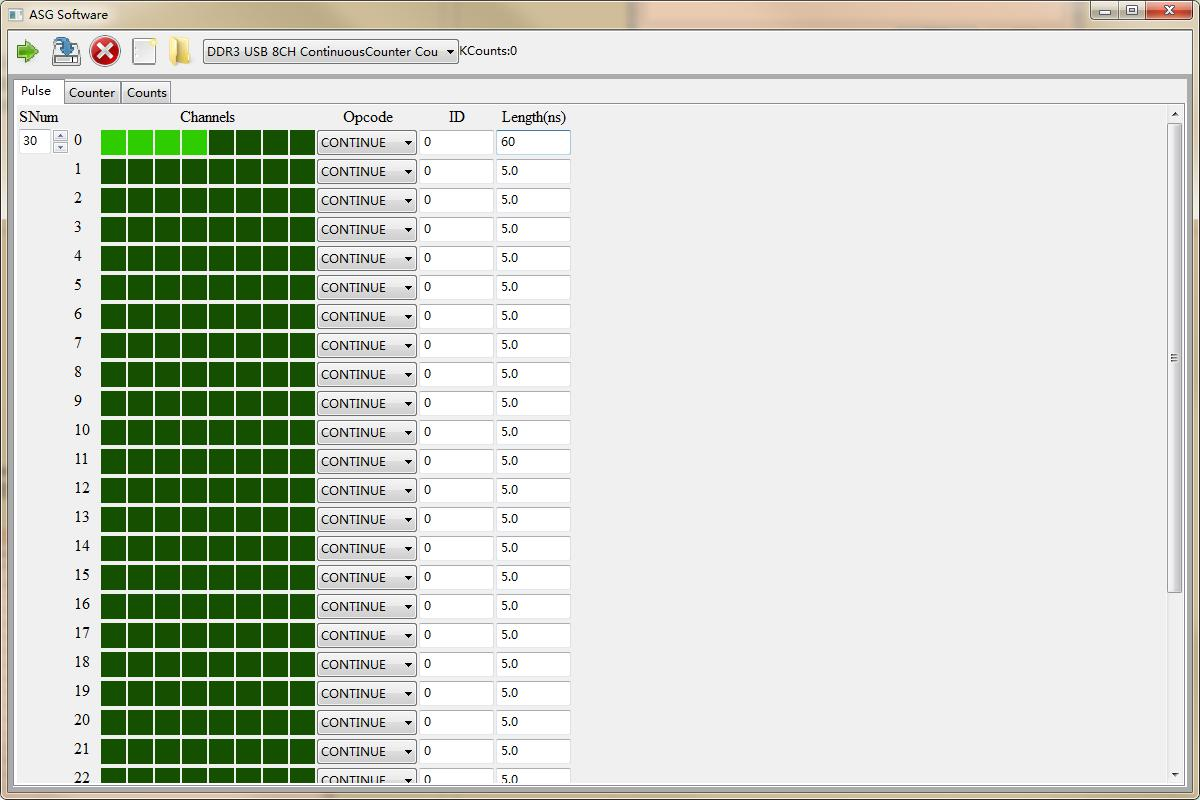
\includegraphics[width=11cm,height=9cm]{fig4_2}
\caption{自定义方波序列}
\end{figure}

\section{\heiti 定义方波序列注意事项}
\noindent 1. 每个通道的单个方波序列高低电平时间必须在5 ns至2.6 s以内。例如用户定义的方波序列中存在宽度小于5 ns的情况,则为非法输入,如图4-3。
\begin{figure}[H]
\centering
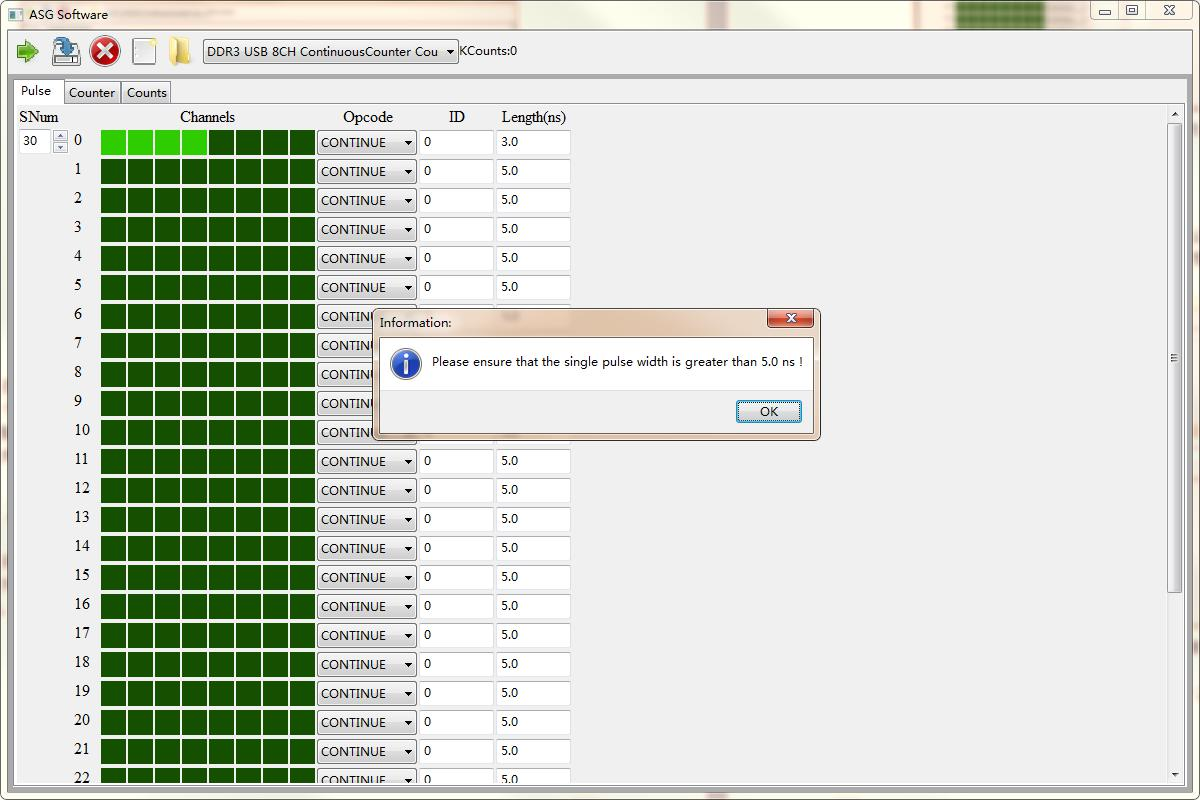
\includegraphics[width=11cm,height=9cm]{fig4_3}
\caption{宽度小于5 ns的非法方波序列输入}
\end{figure}

\newpage
\noindent 2. 若用户定义的方波序列中存在宽度大于2.6 s的情况,亦为非法输入,如图4-4。
\begin{figure}[ht]
\centering
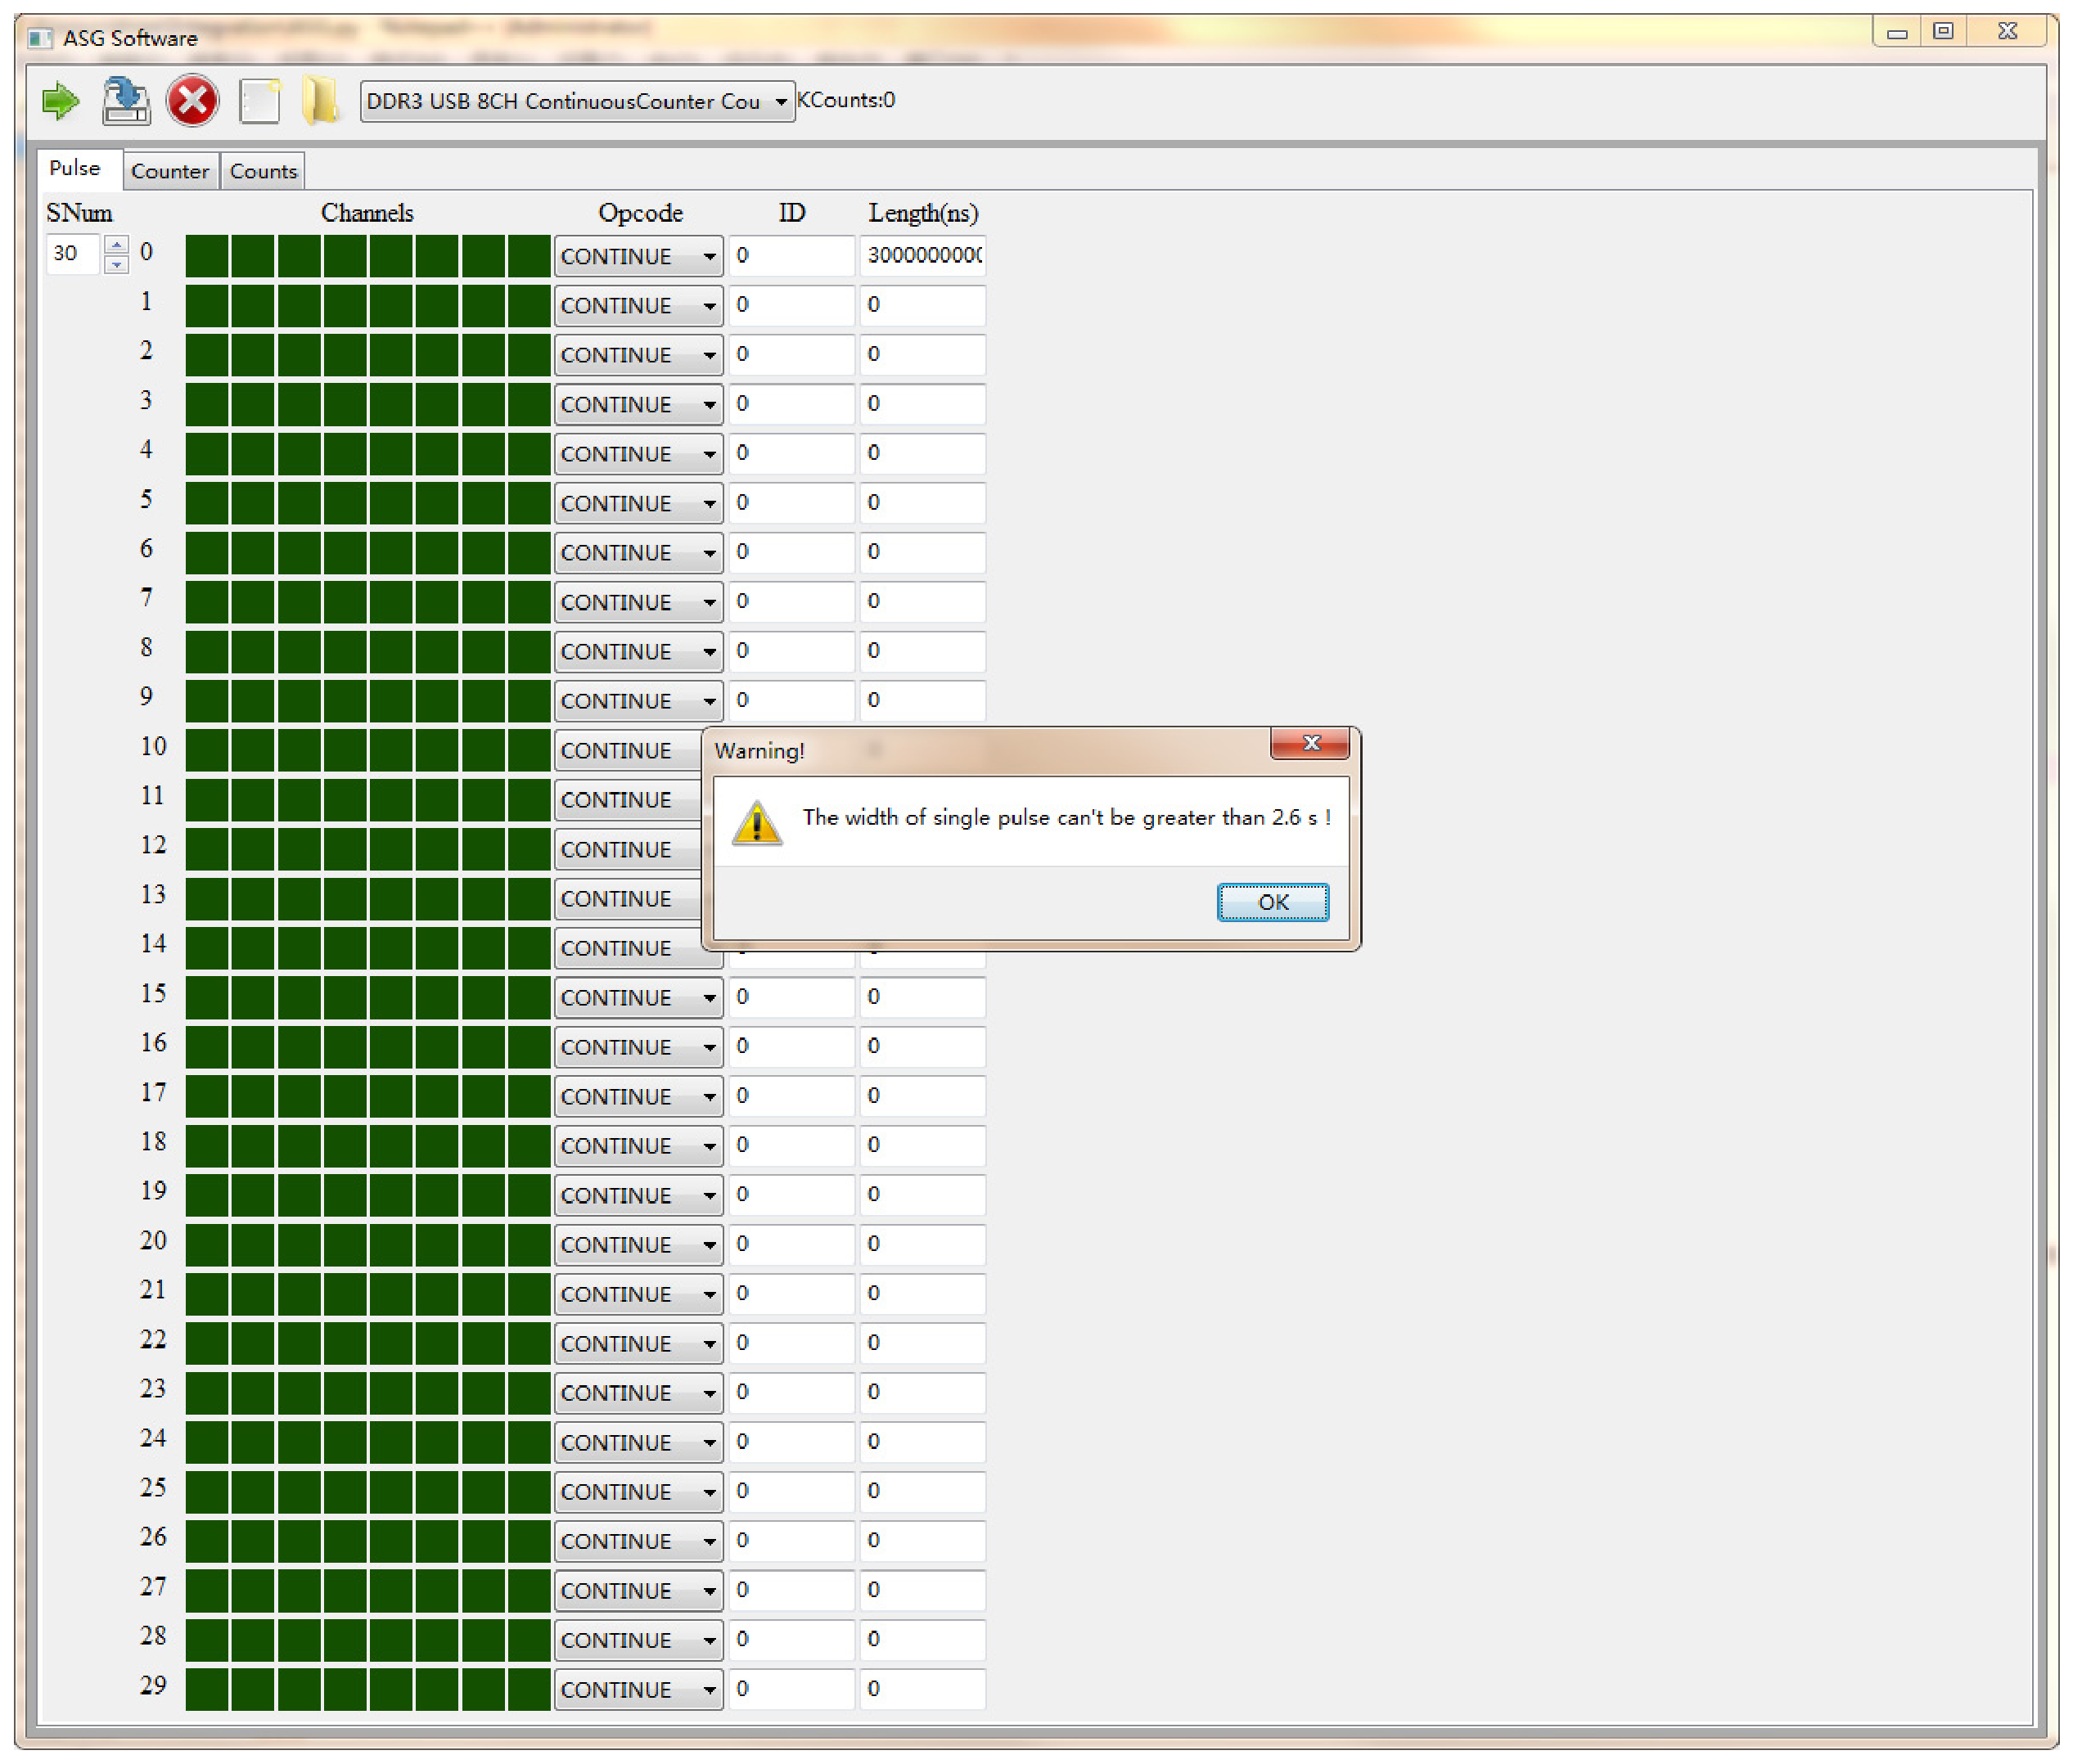
\includegraphics[width=11cm,height=8cm]{fig4_4}
\caption{宽度大于2.6 s的非法方波序列输入}
\end{figure}

\noindent 3. 用户定义的方波序列宽度必须是0.05 ns的整数倍,若存在非0.05 ns整数倍的情况,亦为非法输入,如图4-5。
\begin{figure}[H]
\centering
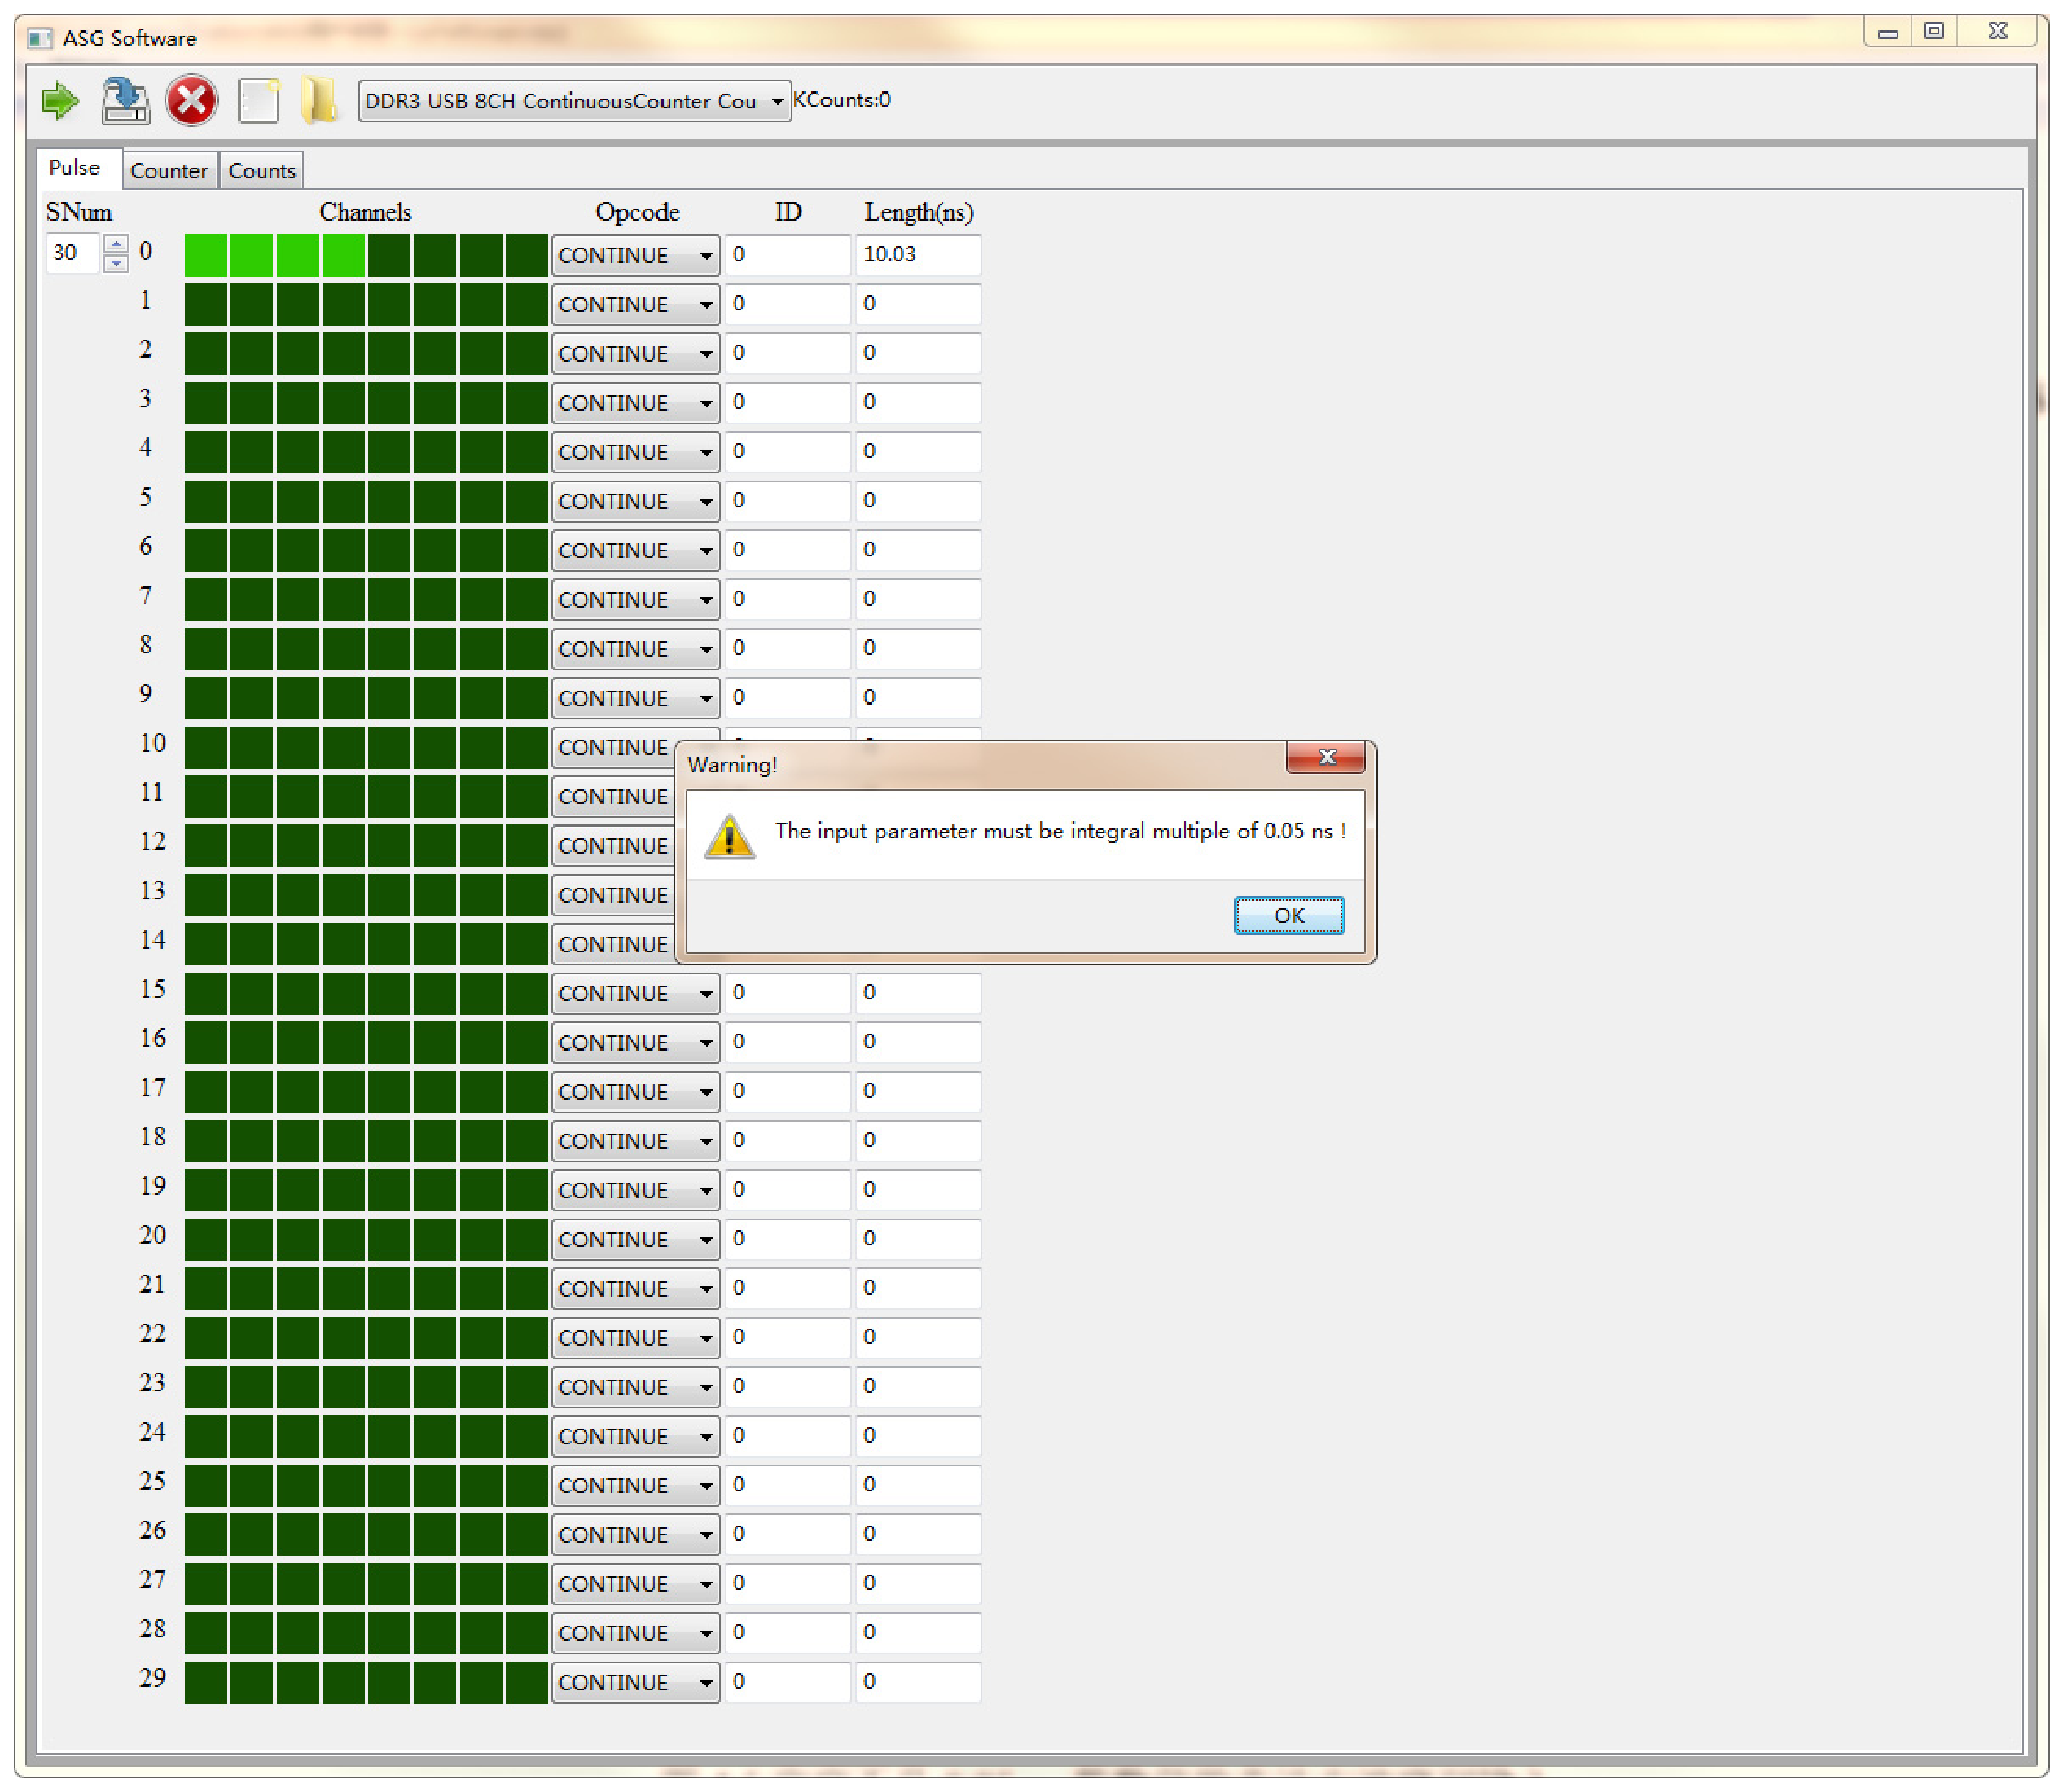
\includegraphics[width=11cm,height=8cm]{fig4_5}
\caption{宽度不是0.05 ns整数倍的非法方波序列输入}
\end{figure}

\section{\heiti{定义}Counter\heiti{序列}}
用户选择“Counter”选项卡进入定义Counter序列界面,如图4-6。左侧为显示计数结果的坐标图。用户可根据中间绿色方框的状态以及“Length”的长度来定义任意的Counter序列。同方波序列输入,绿色方框被点亮代表高电平,未点亮代表低电平。
\begin{figure}[ht]
\centering
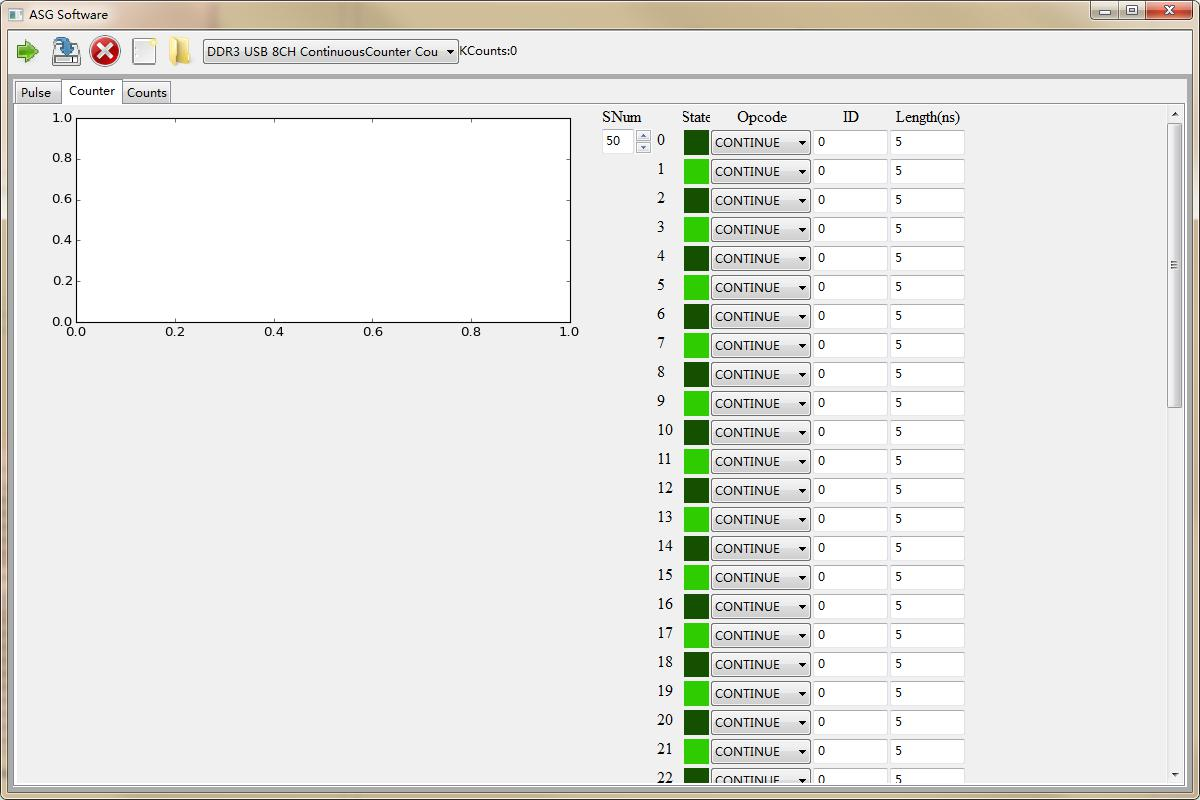
\includegraphics[width=10cm,height=8cm]{fig4_6}
\caption{Counter 界面}
\end{figure}

\section{\heiti{定义}Counter\heiti{序列注意事项}}
\noindent 1. 单个Counter序列的高低电平时间必须在5 ns至5000 s以内。例如用户定义的Counter序列中存在宽度小于5 ns的情况,则为非法输入,如图4-7。
\begin{figure}[ht]
\centering
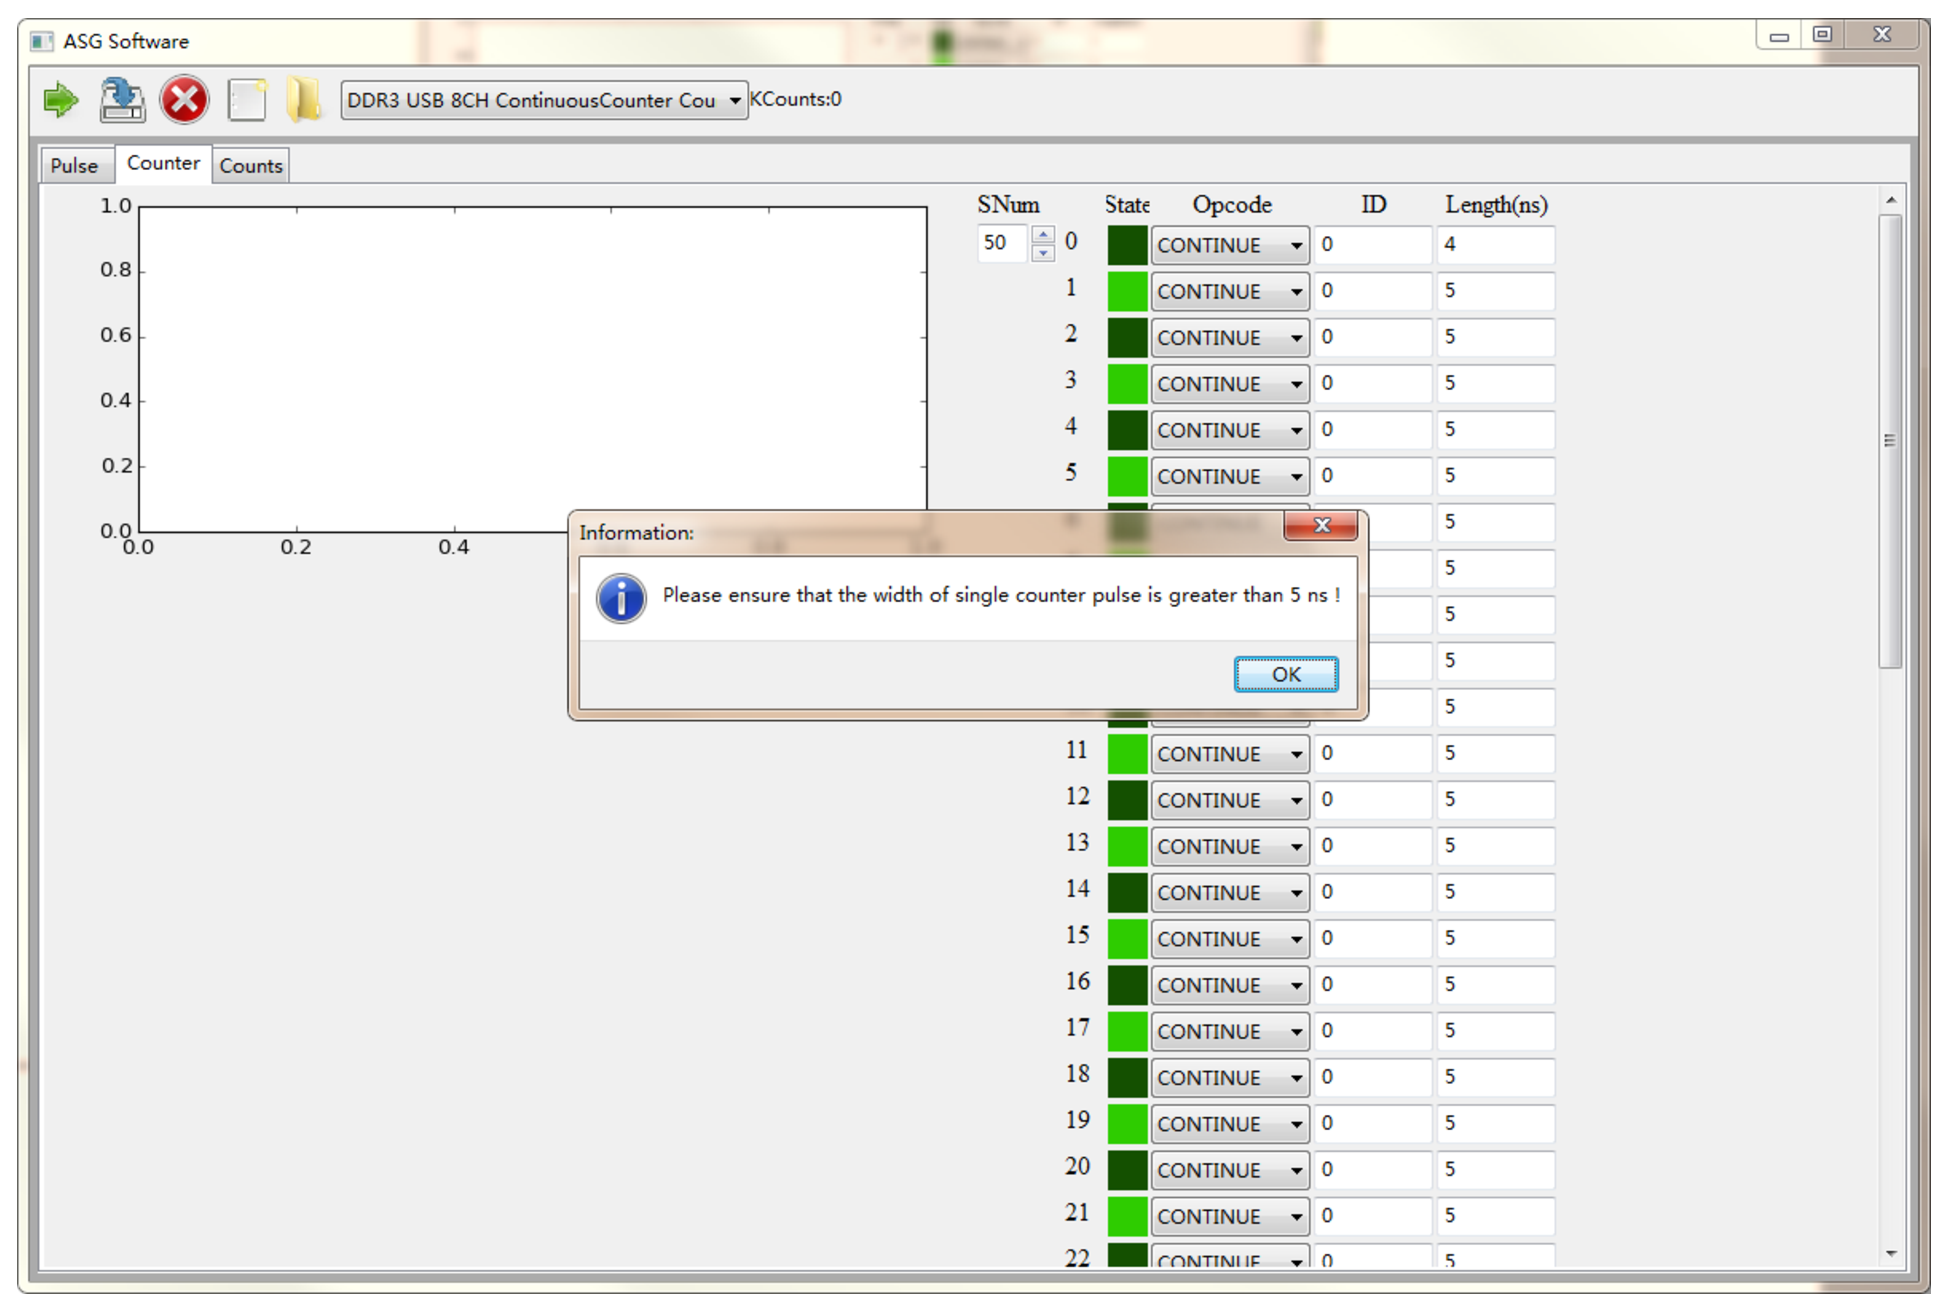
\includegraphics[width=10cm,height=8cm]{fig4_7}
\caption{宽度小于5 ns的非法Counter序列输入}
\end{figure}

\newpage
\noindent 2. 若用户定义的方波序列中存在宽度大于5000 s的情况,亦为非法输入,如图4-8。
\begin{figure}[ht]
\centering
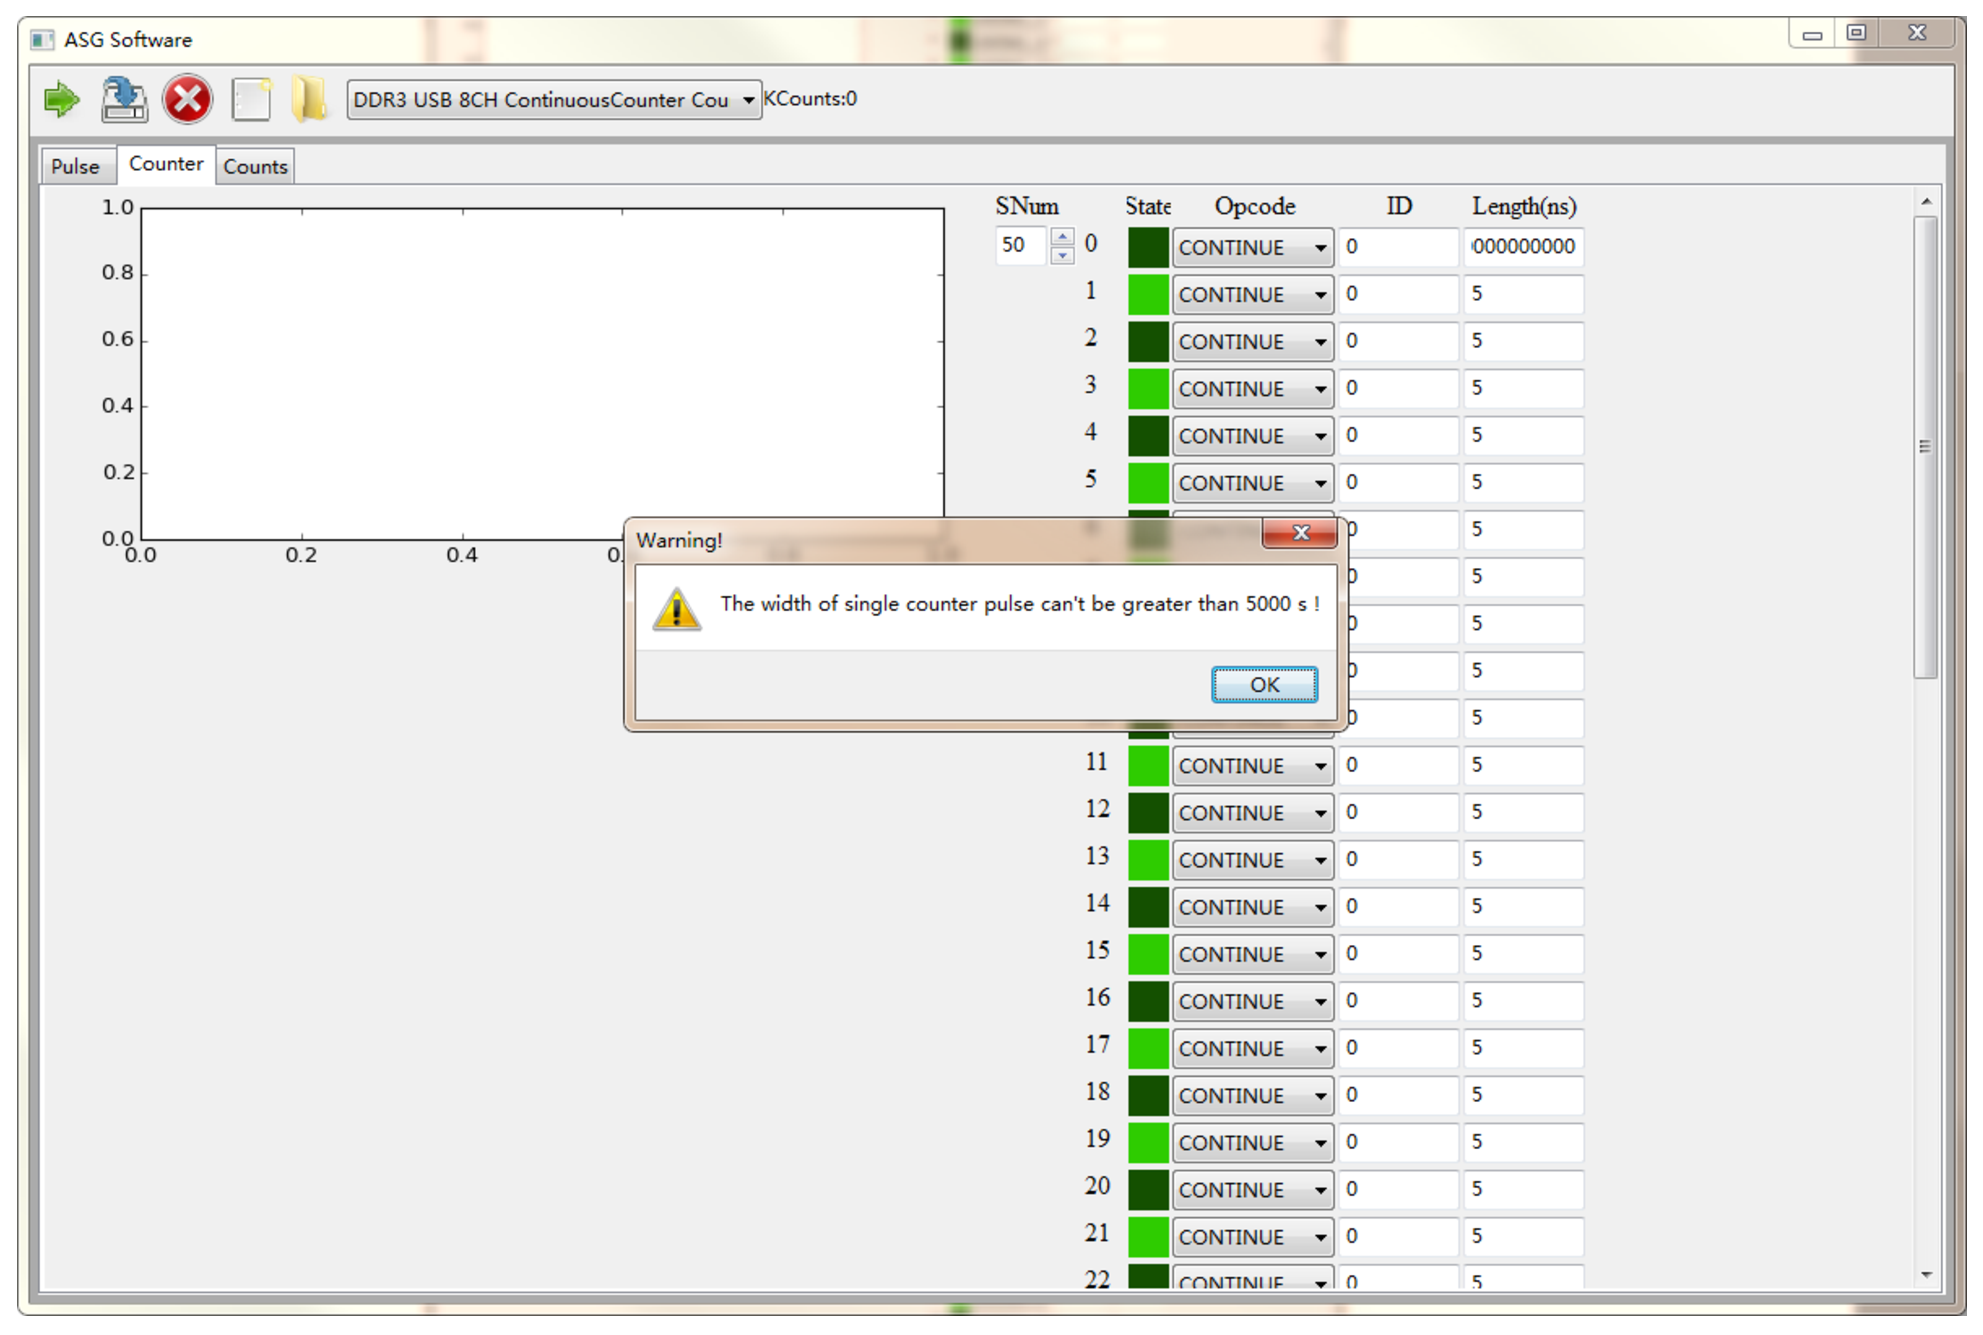
\includegraphics[width=10cm,height=7.5cm]{fig4_8}
\caption{宽度大于5000 s的非法Counter序列输入}
\end{figure}

\noindent 3. 用户定义的Counter序列宽度必须是5 ns的整数倍,若存在非5 ns整数倍的情况,亦为非法输入,如图4-9。
\begin{figure}[ht]
\centering
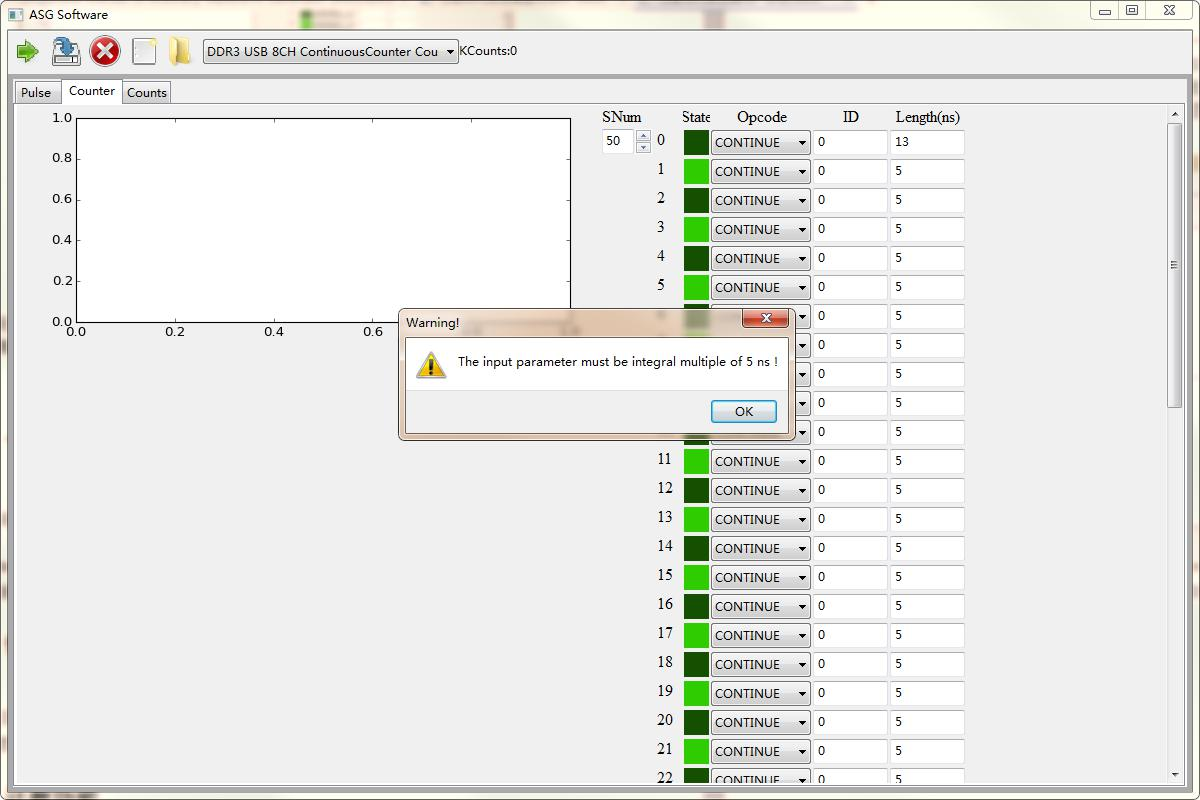
\includegraphics[width=10cm,height=7.5cm]{fig4_9}
\caption{宽度非5 ns整数倍的非法Counter序列输入}
\end{figure}

\section{\heiti 下载与播放方波序列}
用户点击“Download”按钮

\includegraphics{download},可将自定义方波序列数据下载到硬件中。点击“Start”按钮

\includegraphics{start},可使仪器各输出通道开始同步播放自定义的方波序列。将输出通道用同轴线接到示波器上可以看到输出的方波序列。

\section{\heiti 停止计数与播放方波序列}
当仪器正在播放方波序列并计数时,可以通过点击“Stop”按钮
\includegraphics{stop}使仪器停止播放方波序列并停止计数。

\section{\heiti 计数功能}
Counter计数功能是指用户可以定义Counter序列,然后得到在Counter序列高电平时间内输入信号的计数结果。当由外部信号输入Counter通道时,用户可以在软件的Counter界面看到计数结果。计数结果显示在界面左侧的坐标图中。

\section{\heiti 连续计数功能}
连续计数是指用户可以利用软件获得在一段时间内的输入信号计数结果。连续计数功能主界面如图4-10所示。右上方文本输入框为用户自定义的连续计数时间(单位为秒),右下方显示数字为输入计数通道内的信号频率(单位为kHz),左侧坐标图显示连续计数结果随时间的变化图。
\begin{figure}[ht]
\centering
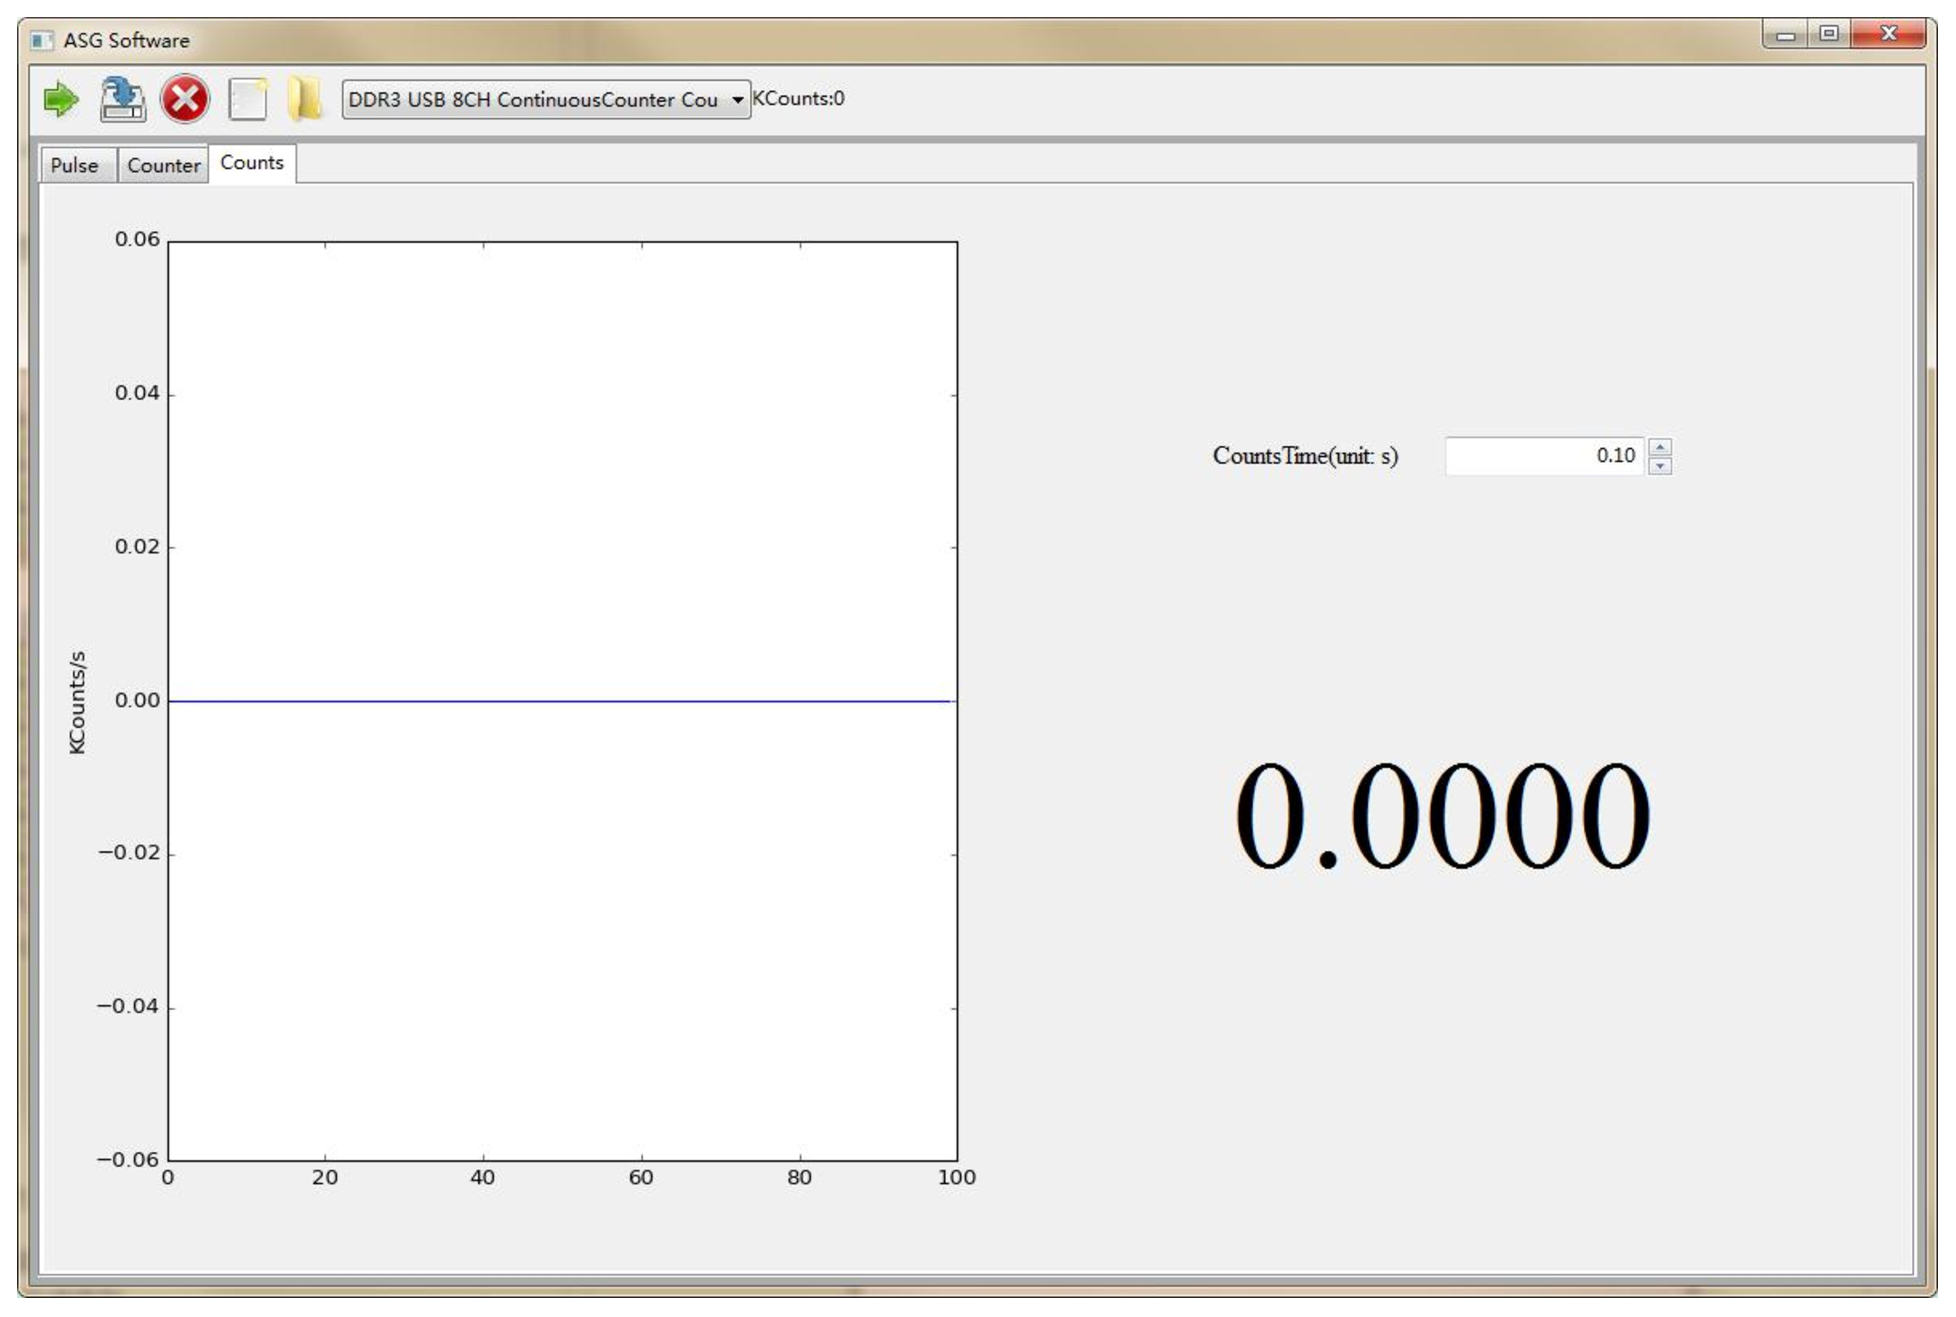
\includegraphics[width=10cm,height=7.5cm]{fig4_10}
\caption{连续计数主界面}
\end{figure}

